\section{Gaussian Channels with Bandlimited, Parallel, Colored Noise}
1. AWGN
$$Y=X+Z, Z\sim\mathcal{N}(0,N), \mathbb{E}(X^2)\leq P\Rightarrow C=\dfrac{1}{2}\log\left(1+\dfrac{P}{N}\right)$$

2. Bandwith Limited Channel \\
Bandwidth: 在正半轴的跨度. 由于实信号的频谱关于y轴对称, 所以只考虑正半轴即可. \\
如在下图两个信号的频谱图中, 左边信号的Bandwidth为$W$, 右边信号的Bandwidth为$2W$.
\begin{figure}[htbp]
    \centering
    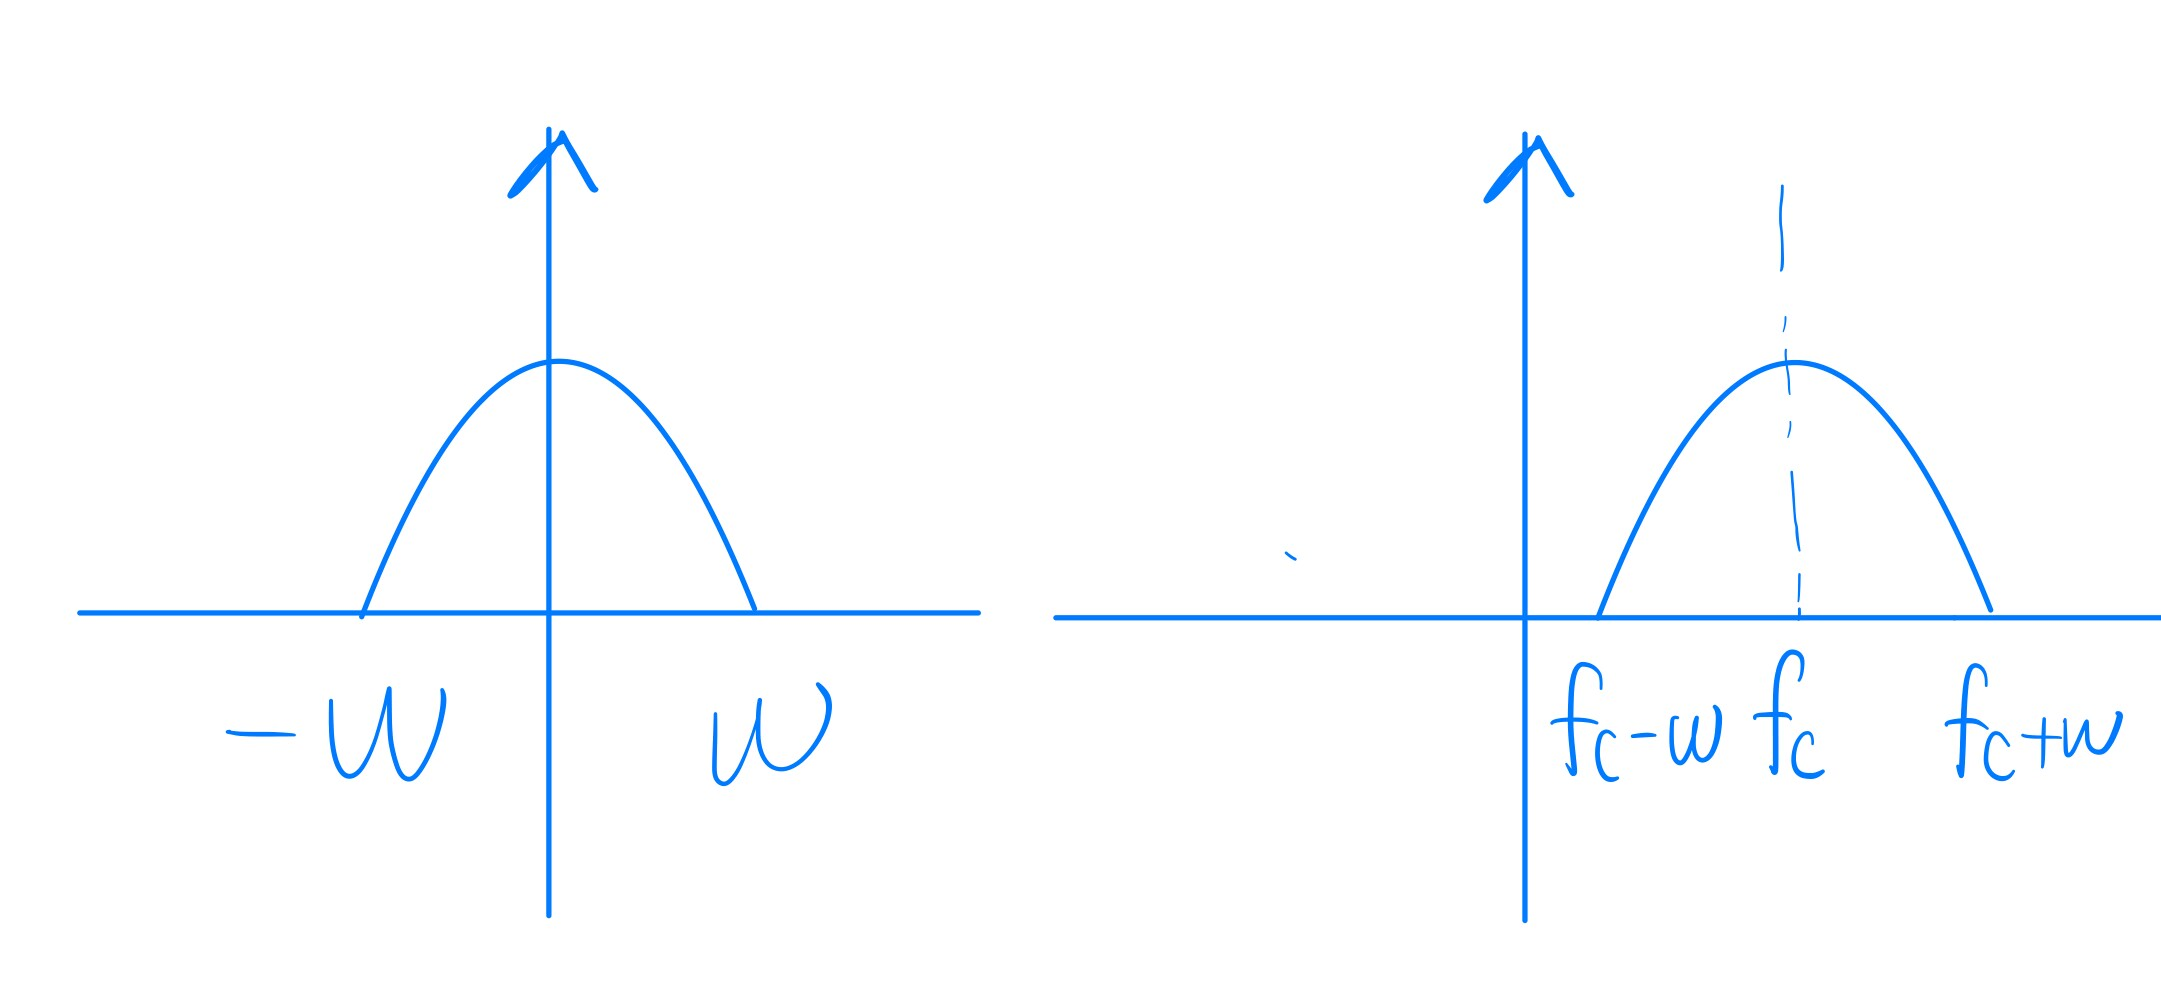
\includegraphics[width=0.6\textwidth]{./figures/chapter7/bandwidth.png}
\end{figure}

Bandwidth Limited Channel: 在信号传输时有Bandwidth限制, 信号的频谱在$W$范围内.
$$Y(t)=X(t)+Z(t)$$
其中信号的能量有限制: $\mathbb{E}(X(t)^2)\leq P$, $Z(t)$为 Guassian Noise with power spectral density(PSD) $\dfrac{N_0}{2}$.

在传输信号时, 对信号做量化: $x[n]=x(nT_s)$, 其中$T_s$为采样周期, $f_s=\dfrac{1}{T_s}$为采样频率. 由 Nyquist 采样定理, 有 $f_s\geq 2W$. \\
Take $T_s=\dfrac{1}{2W}$, 则在$T$时间内的采样点的个数为$2WT$. $T$时间内的总能量为$PT$. 所以 $\mathbb{E}(X_i^2)=\dfrac{PT}{2WT}=\dfrac{P}{2W}$.
\begin{figure}[htbp]
    \centering
    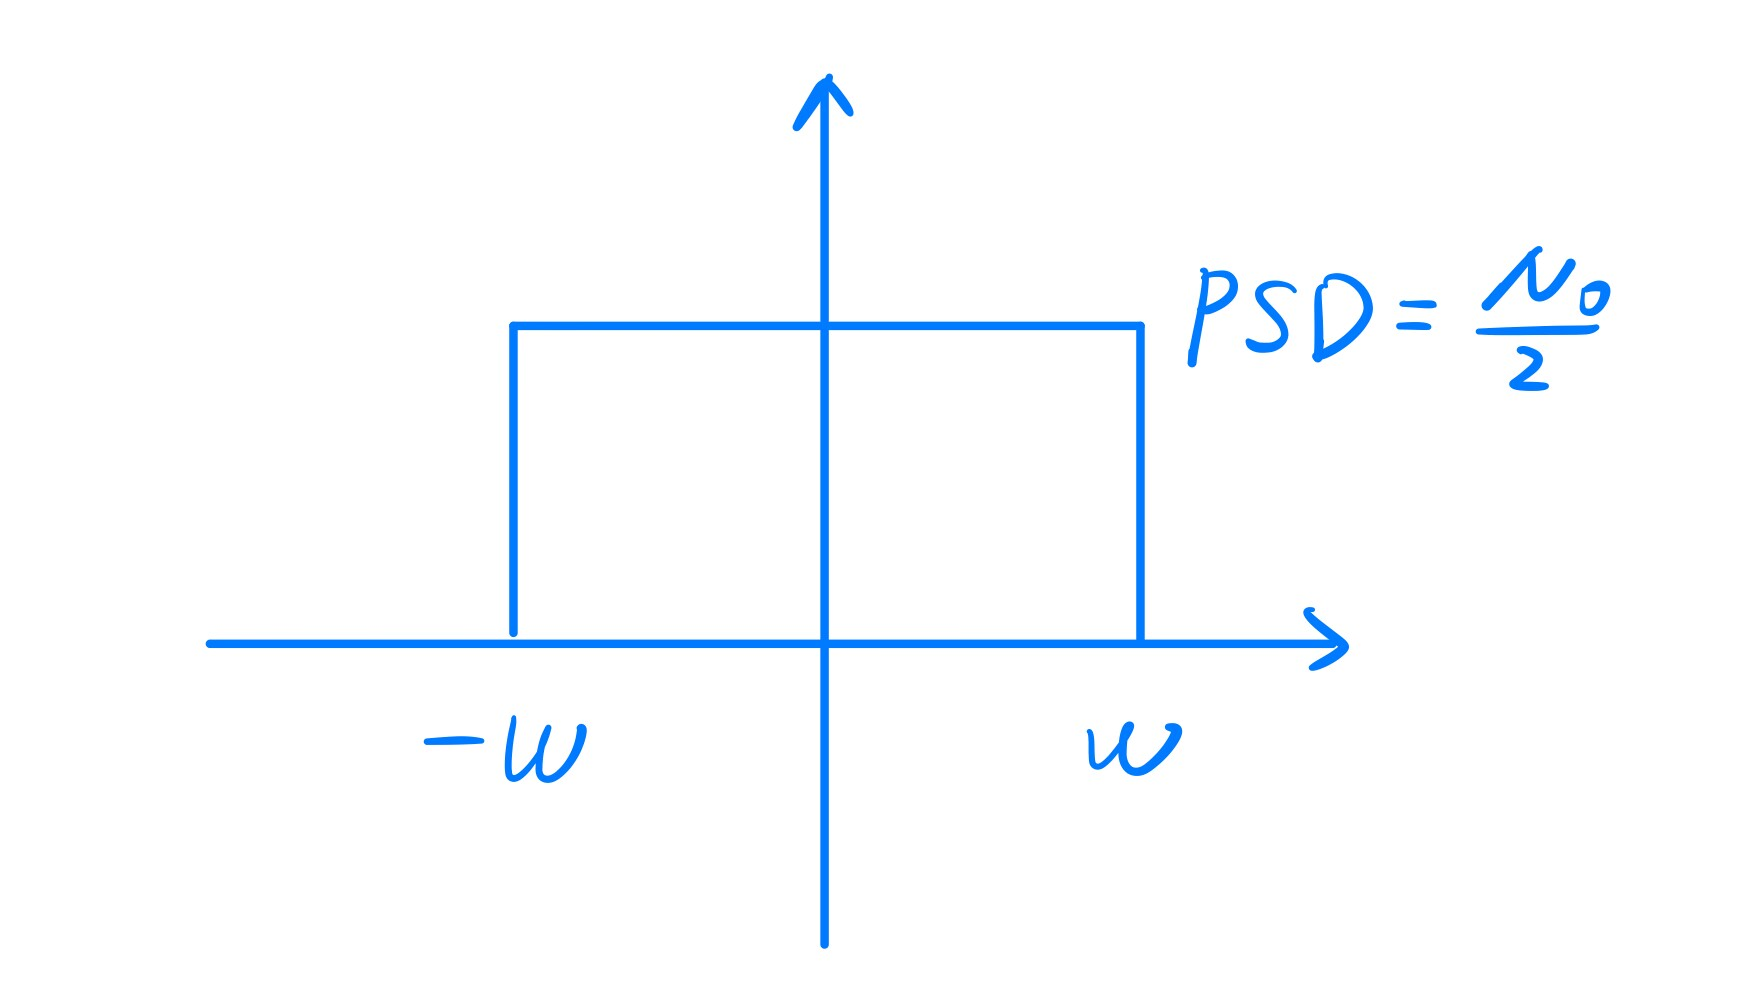
\includegraphics[width=0.5\textwidth]{./figures/chapter7/noise.png}
\end{figure}

Noise的power spectral density 为 $\dfrac{N_0}{2}$ watts/hertz, bandwidth 为 $W$ hertz, 所以噪声的功率为 $\dfrac{N_0}{2}\cdot 2W=N_0W$ watts. 所以平均每个噪声sample的能量为 $\mathbb{E}(Z_i^2)=\dfrac{N_0WT}{2WT}=\dfrac{N_0}{2}$.

由 1. AWGN 的结论, 我们可以得到每个sample的信道容量:
$$C=\dfrac{1}{2}\log\left(\dfrac{1+\frac{P}{2W}}{\frac{N_0}{2}}\right)=\dfrac{1}{2}\log\left(1+\dfrac{P}{N_0W}\right) \text{bits per sample}$$
由于$T=1s$内有$2W\cdot 1$个sample, 所以信道容量为
$$C=2W\cdot\dfrac{1}{2}\log\left(1+\dfrac{P}{N_0W}\right)=W\log\left(1+\dfrac{P}{N_0W}\right) \text{bits per second}$$
几个极端情况: \\
1. $P\to \infty$, $C\to +\infty$ \\
2. $W\to \infty$, $C\to \dfrac{P}{N}\log e$ \\
增加传输功率确实可以无限制增加信道容量, 但是增加带宽会达到瓶颈, 这个瓶颈也能和 $SNR=\dfrac{P}{N_0}$ 相对应.

3. Parallel AWGN
\begin{figure}[htbp]
    \centering
    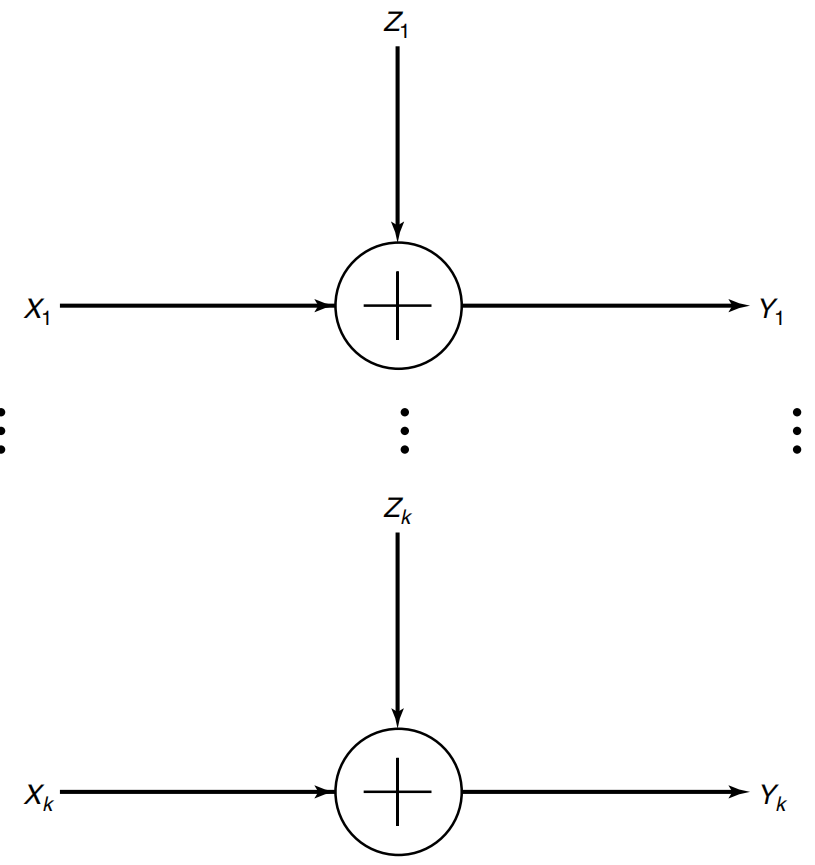
\includegraphics[width=0.5\textwidth]{./figures/chapter7/parallel_Gaussian_channel.png}
\end{figure} \\
如上图, $Y_i=X_i+Z_i, i=1,..,k$, $Z_i\sim \mathcal{N}(0,N_i), Z_i\perp Z_j, \mathbb{E}\left[\sum\limits_{i=1}^k X_i^2\right]\leq P$. \\
则Parallel AWGN 信道的容量为
$$C=\max_{f(x_1,\ldots,x_k):\sum\limits_{i=1}^k \mathbb{E}(X_i^2)\leq P} I(X_1,\ldots,X_k;Y_1,\ldots,Y_k)$$
假设每个$X_i$的能量上限为$P_i$, i.e. $\mathbb{E}(X_i^2)\leq P_i, \sum\limits_{i=1}^k P_i\leq P$, 则有
\begin{align*}
I(X_1,\ldots,X_k;Y_1,\ldots,Y_k) &= h(Y_1,\ldots,Y_k) - h(Y_1,\ldots,Y_k|X_1,\ldots,X_k) \\
&= h(Y_1,\ldots,Y_k) - h(Z_1,\ldots,Z_k) \\
&= h(Y_1,\ldots,Y_k) - \sum_{i=1}^k h(Z_i) \\
&\leq \sum_{i=1}^k \left(h(Y_i) - h(Z_i)\right) \qquad \text{(conditioning reduces entropy)} \\
&= \sum_{i=1}^k I(X_i;Y_i) \qquad\qquad\quad (h(Z_i)=h(Z_i|X_i)=h(Y_i|X_i)) \\
&\leq \sum_{i=1}^k \dfrac{1}{2}\log\left(1+\dfrac{P_i}{N_i}\right) \qquad \text{(AWGN channel capacity)}
\end{align*}
当且仅当$Y_i\perp Y_j$, i.e. $X_i\perp X_j$, 且$X_i\sim\mathcal{N}(0,P_i)$时取等. 所以接下来的问题就是如何分配$P_i$, 使整体的信道容量最大. 我们可以转化成一下的优化问题:
$$
\begin{aligned}
\underset{P_1, \ldots, P_k}{\text{minimize}}\;\; & -\dfrac{1}{2}\sum_{i=1}^k \ln \left(1+\frac{P_i}{N_i}\right) \\
\text { subject to } & \sum_{i=1}^k P_i=P \\
& -P_i \leq 0, i=1, \ldots, k
\end{aligned}
$$
So let $\lambda\in\mathbb{R}, \pmb \mu\in\mathbb{R}^k$ respectively be the multiplier of the equality constrain and inequality constrains, so $\pmb \mu\succeq 0$. And the Lagrangian function is:
\begin{align*}
\mathcal{L}(\pmb p, \lambda, \pmb \mu) &= -\dfrac{1}{2}\sum_{i=1}^k \ln \left(1+\frac{P_i}{N_i}\right) + \lambda\left(\sum_{i=1}^k P_i-P\right) - \pmb \mu^T\pmb p \\
\dfrac{\partial \mathcal{L}}{\partial P_i} &= \dfrac{1}{2}\cdot\dfrac{-1}{N_i+ P_i} + \lambda - \mu_i, \quad i=1,\ldots,k \\
\dfrac{\partial \mathcal{L}}{\partial P_i} = 0 &\Rightarrow P_i^* = \dfrac{1}{2}\cdot\dfrac{1}{\lambda-\mu_i} - N_i, \quad i=1,\ldots,k
\end{align*}

we can get the KKT conditions:
$$\left\{
\begin{aligned}
\text{Primal feasibility:} &\quad
\left\{
\begin{aligned}
&\sum_{i=1}^k P_i^* = P \\
&P_i^* \geq 0, \quad i=1,\ldots,k
\end{aligned}
\right. \\
\text{Dual feasibility:} &\quad \pmb \mu^* \succeq 0 \\
\text{Complementary slackness:} &\quad \mu_i^* P_i^* = 0, \quad i=1,\ldots,k \\
\text{Stationarity:} &\quad \dfrac{\partial \mathcal{L}}{\partial P_i} = 0 \Rightarrow P_i^* = \dfrac{1}{2}\cdot\dfrac{1}{\lambda^*-\mu_i^*} - N_i, \quad i=1,\ldots,k
\end{aligned}
\right.$$

With KKT condition, we can get the optimal solution: \\
First of all, we define $\dfrac{1}{2\lambda^*} \textcolor{red}{\triangleq \nu}$. Then we have: \\
<1> If $P_i^*=0$, then from the stationarity condition, we have $\mu_i^* = \dfrac{1}{2\nu} - \dfrac{1}{2N_i}$. \\
And from the dual feasibility condition, we have $\mu_i^*\geq 0$, so we have $\nu\leq N_i$. \\
<2> If $P_i^*\neq 0$, then from the complementary slackness condition, i.e. $\mu_i^* = 0$. \\
And from the stationarity condition, we have $P_i^* = \nu - N_i$. \\
And from the primal feasibility condition, we have $P_i^* \geq 0$, and since $P_i^*\neq 0$, so we have
$$P_i^* = \nu - N_i > 0 \Leftrightarrow \nu < N_i$$

So above all, we can get that
$$P_i^* = \left\{
\begin{aligned}
&0, &&\quad \nu \leq N_i \\
&\nu - N_i, &&\quad \nu > N_i
\end{aligned}
\right.$$
Which means that
$$P_i^* = \max\left\{0, \nu - N_i\right\} = (\nu - N_i)_+$$
And from the primal feasibility condition, we have
$$\sum_{i=1}^k P_i^* = P$$
So with some methods, such as the bisection method, we can get the value of $\nu$ with the above equation. And after calculating $\nu$, we can get the optimal solution of $P_i^*$. \\
And the optimal value of the origin problem is
\begin{align*}
\text{obj} &= \dfrac{1}{2}\sum_{i=1}^k \ln \left(1+\frac{P_i^*}{N_i}\right) \\
&= \dfrac{1}{2}\sum_{i=1}^k \ln \left(1+\frac{\max\left\{0, \nu - N_i\right\}}{N_i}\right)
\end{align*}

这个方法也叫做 Water Filling Algorithm. 我们可以用二分或其他方法得到$\nu$, 然后由$P_i=(\nu-N_i)_+$得到$P_i$, 最后找到那个能够满足$\sum\limits_{i=1}^k P_i=P$的$\nu$即可. \\
可以按照下图理解, 其中$\nu$为水线, noise($N_i$)为石头, 水深为$P_i$. $N_i$越大, $P_i$越小.
\begin{figure}[htbp]
    \centering
    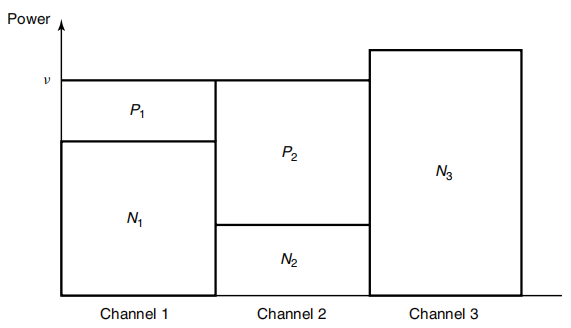
\includegraphics[width=0.75\textwidth]{./figures/chapter7/water_filling.png}
\end{figure}

4. AWGN with correlated noise \\
Lemma: Hadamard's Inequality. 对于任意$n$阶\textcolor{red}{半正定}方阵$A=(a_{ij})_{n\times n}$:
$$|A| \leq \prod_{i=1}^n a_{ii}$$
当$A$为对角阵时取等. \\
之前噪声都是独立的, 若增加噪声直接的相关性: $Z^n=(Z_1,\ldots,Z_n)\sim\mathcal{N}(0,\bK_Z)$
由于$Z_i$有相关性, 所以考虑$X^n$也有相关性, coviance matrix 为 $\bK_X$. 也可以理解为\textbf{使 channels with memory}. 在with memory的情况下, 能量约束变为了$\dfrac{1}{n}\mathbb{E}(X_i^2)\leq P\Rightarrow \dfrac{1}{n}\text{Tr}(\bK_X)\leq P$.
$$\Cov(Y_i,Y_j)=\Cov(X_i+Z_i,X_j+Z_j)=\Cov(X_i,X_j)+\Cov(Z_i,Z_j)\Rightarrow \bK_Y=\bK_X+\bK_Z$$
所以
\begin{align*}
I(X^n;Y^n) &= h(Y^n) - h(Y^n|X^n) \\
&= h(Y^n) - h(Z^n) \\
&\leq \dfrac{1}{2}\log\left((2\pi e)^n|\bK_Y|\right) - \dfrac{1}{2}\log\left((2\pi e)^n|\bK_Z|\right)
\end{align*}
由于$\bK_Z$是coviance matrix, 一定是对称阵, 所以可以正交对角化, 写作 $\bK_Z=Q\Lambda Q^{\top}$, where $Q^{\top}Q=I$, so:
\begin{align*}
|\bK_X + \bK_Z| &= |\bK_X + Q\Lambda Q^{\top}| \\
&= |Q(Q^{\top}\bK_XQ+\Lambda)Q^{\top}| \\
&= |Q^{\top}\bK_XQ+\Lambda|
\end{align*}
Let $A=Q^{\top}\bK_XQ$, then:
$$\Tr(A)=\Tr(Q^{\top}\bK_XQ)=\Tr(\bK_XQQ^{\top})=\Tr(\bK_X)\leq nP$$
由 Hadamard inequality:
$$|\bK_X + \bK_Z| = |A+\Lambda| \leq \prod\limits_{i=1}^n (\lambda_i + a_{ii})$$
和往常一样, 应用 Water Filling Algorithm, $a_{ii}=(\nu-\lambda_i)_+$, $\nu$使得$\Tr(A)=\sum\limits_{i=1}^n (\nu-\lambda_i)_+=nP$即可. \\
所以最终的信道容量为
$$C=\dfrac{1}{2}\log\left(\dfrac{\prod_{i=1}^n (\lambda_i + (\nu-\lambda_i)_+)}{|\bK_Z|}\right)$$
其中 $\sum\limits_{i=1}^n (\nu-\lambda_i)_+=nP$, $\lambda_i$为$\bK_Z$的特征值, $A=Q^{\top}\bK_XQ$, $Q$为$\bK_Z$正交对角化矩阵.


5. Gaussian Channels with Colored Noise \\
Channels in which the noise forms a stationary stochastic process, the input signal should be chosen to be a Gaussian process with a spectrum that is large at frequencies where the noise spectrum is small.
\begin{figure}[htbp]
    \centering
    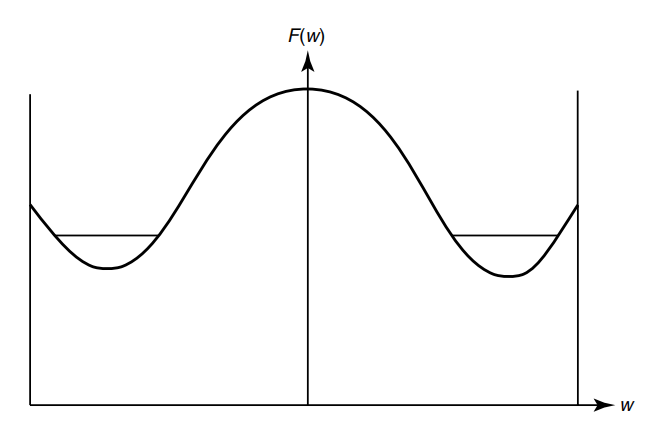
\includegraphics[width=0.5\textwidth]{./figures/chapter7/water_filling_spectrum.png}
\end{figure}

用频域上的 water-filling, $\nu$为水线, 满足 $\int (\nu-N(f))_+ df=P$即可.
$$C=\int_{-\pi}^{\pi} \dfrac{1}{2}\log\left(1+\dfrac{(\nu-N(f))_+}{N(f)}\right) df$$

6. Feedback: $Y_{i+1}$的产生有$Y_i$参与
\begin{figure}[htbp]
    \centering
    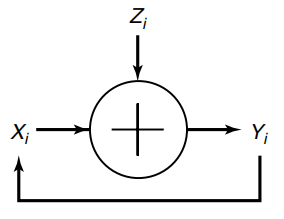
\includegraphics[width=0.3\textwidth]{./figures/chapter7/feedback.png}
\end{figure}

无论是否feedback, Channel capacity均为 $C=\dfrac{1}{2}\log\left(\dfrac{\bK_{X+Z}}{\bK_Z}\right)$, 但是without feedback有$\bK_{X+Z}=\bK_X+\bK_Z$. \\
Memoryless Channel capacity: $C_{noFB}$, Channel without feedbeck $C_{FB}$, 满足bound:
\begin{align*}
C_{FB} &\leq C_{noFB} + \dfrac{1}{2} \\
C_{FB} &\leq 2C_{noFB}
\end{align*}
Without memory $p_e^{(n)}$ exponentially $\searrow 0$, with memory double exponentially $\searrow 0$, 可以更快的收敛到0, more robust.